\documentclass[12pt,letterpaper]{article}
\usepackage[utf8]{inputenc}
\usepackage[spanish, es-tabla]{babel}
\usepackage[version=3]{mhchem}
\usepackage[journal=jacs]{chemstyle}
\usepackage{amsmath}
\usepackage{amsfonts}
\usepackage{amssymb}
\usepackage{makeidx}
\usepackage{xcolor}
\usepackage[stable]{footmisc}
\usepackage[section]{placeins}
\usepackage{listings}
\usepackage{siunitx}
\sisetup{mode=text, output-decimal-marker = {,}, per-mode = symbol, qualifier-mode = phrase, qualifier-phrase = { de }, list-units = brackets, range-units = brackets, range-phrase = --}
\DeclareSIUnit[number-unit-product = \;] \atmosphere{atm}
\DeclareSIUnit[number-unit-product = \;] \pound{lb}
\DeclareSIUnit[number-unit-product = \;] \inch{"}
\DeclareSIUnit[number-unit-product = \;] \foot{ft}
\DeclareSIUnit[number-unit-product = \;] \yard{yd}
\DeclareSIUnit[number-unit-product = \;] \mile{mi}
\DeclareSIUnit[number-unit-product = \;] \pint{pt}
\DeclareSIUnit[number-unit-product = \;] \quart{qt}
\DeclareSIUnit[number-unit-product = \;] \flounce{fl-oz}
\DeclareSIUnit[number-unit-product = \;] \ounce{oz}
\DeclareSIUnit[number-unit-product = \;] \degreeFahrenheit{\SIUnitSymbolDegree F}
\DeclareSIUnit[number-unit-product = \;] \degreeRankine{\SIUnitSymbolDegree R}
\DeclareSIUnit[number-unit-product = \;] \usgallon{galón}
\DeclareSIUnit[number-unit-product = \;] \uma{uma}
\DeclareSIUnit[number-unit-product = \;] \ppm{ppm}
\DeclareSIUnit[number-unit-product = \;] \eqg{eq-g}
\DeclareSIUnit[number-unit-product = \;] \normal{\eqg\per\liter\of{solución}}
\DeclareSIUnit[number-unit-product = \;] \molal{\mole\per\kilo\gram\of{solvente}}
\usepackage{cancel}
\usepackage{graphicx}
\usepackage{lmodern}
\usepackage{fancyhdr}
\usepackage[left=4cm,right=2cm,top=3cm,bottom=3cm]{geometry}

\usepackage[backend=bibtex,style=chem-acs,biblabel=dot]{biblatex}
\addbibresource{ref.bib}

\usepackage{titlesec}
\usepackage{enumitem}
\titleformat*{\section}{\bfseries\large}
\titleformat*{\subsection}{\bfseries\normalsize}
\usepackage{float}
\floatstyle{plaintop}
\newfloat{anexo}{thp}{anx}
\floatname{anexo}{Anexo}
\restylefloat{anexo}
\restylefloat{figure}
\usepackage[margin=10pt,labelfont=bf]{caption}
\usepackage{todonotes}
\usepackage[colorlinks=true, 
            linkcolor = blue,
            urlcolor  = blue,
            citecolor = black,
            anchorcolor = blue]{hyperref}

\begin{document}
\renewcommand{\labelitemi}{$\checkmark$}

\renewcommand{\CancelColor}{\color{red}}

\newcolumntype{L}[1]{>{\raggedright\let\newline\\\arraybackslash}m{#1}}

\newcolumntype{C}[1]{>{\centering\let\newline\\\arraybackslash}m{#1}}

\newcolumntype{R}[1]{>{\raggedleft\let\newline\\\arraybackslash}m{#1}}

\begin{center}
	\textbf{\LARGE{Criação da biblioteca de análise e processamento de imagens SAR/PolSAR - Um estudo sobre dados raster e a biblioteca raster disponivel em R.}}\\
	\vspace{7mm}
	\textbf{\large{LaCCAN - Laboratório de computação científica e análise numérica}}\\ 
	\vspace{4mm}
	\textbf{\large{Aluno: John Victor}}\\
	\vspace{4mm}
	\textbf{\large{Orientador: Alejandro Frery}}\\
\end{center}

\vspace{7mm}

\section*{\centering Resumo}

Esse relátorio tem como objetivo elencar os avanços e conhecimentos obtidos durante os ultimos meses no que refere-se aos recursos disponíveis em R com intuito de auxiliar na criação das funções e a biblioteca para processamento e análise de imagens SAR/PolSAR.

\section{Introdução}

O foco inicial da pesquisa foi procurar e analisar os recursos disponíveis em R que pudessem ajudar no resultado final. Além disso, a forma como os dados serão tratados e analisados requer uma certa atenção, pois com uma boa forma de tratamento de dados poderemos garantir em parte a eficiência e a qualidade das funções que serão futuramente desenvolvidas. Enfim, abaixo encontram-se algumas perguntas que foram essenciais durante a busca pelos recursos disponíveis em R.

\begin{itemize}

\item De que forma trataremos os dados?
\item Como trabalhar com uma larga quantidade de dados?

\end{itemize}

\section{Resultados}

\subsection{Tratamento de dados}

No que refere-se a tratamento de dados foi levado em conta as questôes da simplicidade e versatibilidade, desta forma foi encontrado o tipo de dado raster, o qual consiste de uma matriz organizada em linhas e colunas, na qual cada elemento ou célula possui um valor que representa a informação que está sendo tratada no dado. Abaixo, alguns pontos positivos dos dados raster e uma possível representação.

\begin{itemize}

\item Estrutura simples
\item Grande potêncial na analise de dados espaciais e estátisticos
\item A possibilidade de sobreposições rapidas com complexos conjuntos de dados.
\item Amazenar de maneira uniforme linhas, pontos, poligonos e superficies
\item A possibilidade de representar superficies continuas e realizar analise de superficies

\end{itemize}

\begin{figure}
  \centering
  \textbf{Exemplo de representação raster}
   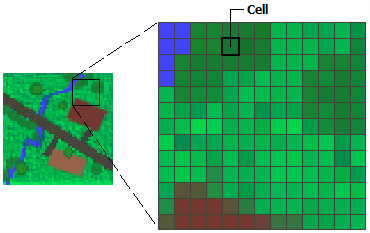
\includegraphics[width=15cm,height=7cm]{Raster.png}
\end{figure}

\subsection{Biblioteca Raster}

É uma biblioteca disponivel em R que possui bastante potêncial no que refere-se ao tratamento de grande quantidade de dados, pois não é necessário carregar todo o conjunto de dados na memória Ram uma vez que é possível trabalhar com arquivos que possuem apenas informações essênciais dos dados como o número de linhas, colunas, o nome do arquivo e a extensão espacial. Abaixo, Alguns recursos disponíveis pela biblioteca:

\begin{itemize}

\item Leitura e escrita de diversos tipos de arquivos raster
\item Plotagem de dados
\item Fácil acesso aos dados do arquivo raster
\item Possui modelos de previsão
\item Raster Algebra e funções de sobreposição de conjunto de dados
\item Criação de Objetos raster diretamente de arquivos
\item Manipulação de grandes quantidades de dados

\end{itemize}

\begin{figure}

\centering
   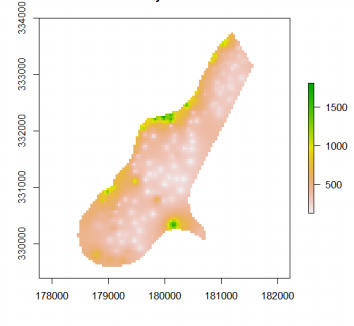
\includegraphics[width=12cm,height=6cm]{RasterLayer.png}
	\caption{Exemplo de plotagem de um RasterLayer retirado de arquivo}
    
\end{figure}

\section{Conclusão}

Desse modo, com os recursos obtidos teremos um ponto de partida mais interessante que dará suporte na criação das funções e da biblioteca final, os futuros esforços serão destinados ao estudo das caracteristicas e o funcionamento das imagens SAR/PolSAR. 

\section*{Referências}

\begin{enumerate}
\item Robert J. Hijmans, Introduction to the ’raster’ package \textbf{2016}
\end{enumerate}

\end{document}